% %% %%%%%%%%%%%%%%%%%%%%%%%%%%%%%%%%%%%%%%%%%%%%%%%%%%%%%%%%%%
% intro-adc.tex
%
% Author:  Mauricio Matamoros
% License: MIT
%
% %% %%%%%%%%%%%%%%%%%%%%%%%%%%%%%%%%%%%%%%%%%%%%%%%%%%%%%%%%%%

%!TEX ROOT=../main.tex
%!TEX ROOT=../references.bib

% CHKTEX-FILE 1
% CHKTEX-FILE 46

Para leer la señal del LM35 se requiere de un Convertidor Analógico Digital o ADC (por sus siglas en inglés: \emph{Digital-Analog Converter}).
Un ADC se elige con base en dos factores clave: su precisión y su tiempo de muestreo.
Debido a que la aplicación del ADC será convertir mediciones de temperatura y los cambios de temperatura son muy lentos,\footnotemark{} puede obviarse el tiempo de muestreo.
En cuanto a la precisión, los convertidores A/D más comunes son de 8 y 10 bits, de los cuales ha de elegirse uno.

La precisión del ADC se calcula tomando en cuenta el rango de operación y la precisión del componente analógico a discretizar.
El LM35 tiene un rango de \degreesC{205}, una diferencial de voltaje $\Delta{}V=10mV/^{o}C$ y una precisión máxima de \degreesC{0.5}, por lo que el sensor entregará un máximo de 2.5V respecto al voltaje de referencia del mismo, con incrementos de 5mV.
Debido a que 256 valores para un rango de \degreesC{205} en incrementos de \degreesC{0.5} (es decir 410 valores) es claramente insuficiente para este sensor, por lo que será conveniente utilizar un convertidor A/D de 10 bits.

Un ADC típico de 10 bits convertirá las señales analógicas entre voltajes de referencia $V_{Ref-}$ y $V_{Ref+}$ como un entero con valores entre 0 y 1023, interpretando los valores $V_{Ref-}$ como 0 lógico y $V_{Ref+}$ como 1023 de manera aproximadamente lineal.
El decir, la lectura obtenida es directamente proporcional al voltaje dentro del rango, estimable mediante la fórmula:

\begin{equation}
V_{out}= value \times \frac{ V_{Ref+} - V_{Ref-} }{ 1024 }
\end{equation}

En una configuración simple, $V_{Ref-}$ y $V_{Ref+}$ se conectan internamente dentro del Arduino a tierra y V\textsubscript{CC} respectivamente. Esto simplifica la fórmula como:

\begin{equation}
V_{out}= value \times \frac{ 5V }{ 1024 } = value \times 0.00488V
\end{equation}

Considerando que el LM35 en rango completo entrega hasta 2.05V ($10mV\times (150 - -55) = 2.05V$) la mayor parte de los 1024 valores jamás serán ocupados.
Es por esto que la mayoría de los convertidores analógico-digital incluyen pines para voltajes de referencia $V_{Ref+}$ y $V_{Ref-}$, para lo cual se hace uso de un divisor de voltaje usando la fórmula:

\begin{equation}
\label{eqn:vdiv}
V_{out}= \frac{ R_2 }{ R_1 + R_2 } \times V_{IN}
\end{equation}

Por ejemplo, supóngase que se utilizará un Arduino UNO alimentado a $5V_{CC}$ que cuenta sólo con un pin voltaje de referencia positivo $V_{Ref+}$, denominado \emph{AREF} según las especificaciones~\Citep{ArduinoWeb}.
Usando un par de resistencias $R_1 = 10k\Omega$ y $R_2 = 12k\Omega$ (véase~\Cref{fig:lm35-arduino}) para generar un voltaje de referencia para un LM35 en configuración típica de rango completo se tendría:

\begin{equation}
V_{AREF}
	= \frac{ 12\Omega }{ 12\Omega + 10\Omega } \times 5V
	= \frac{ 12\cancel{\Omega} }{ 22\cancel{\Omega} } \times 5V
	= \frac{ 60V }{ 22 } = 2.72V
\end{equation}

\begin{figure}
	\centering
	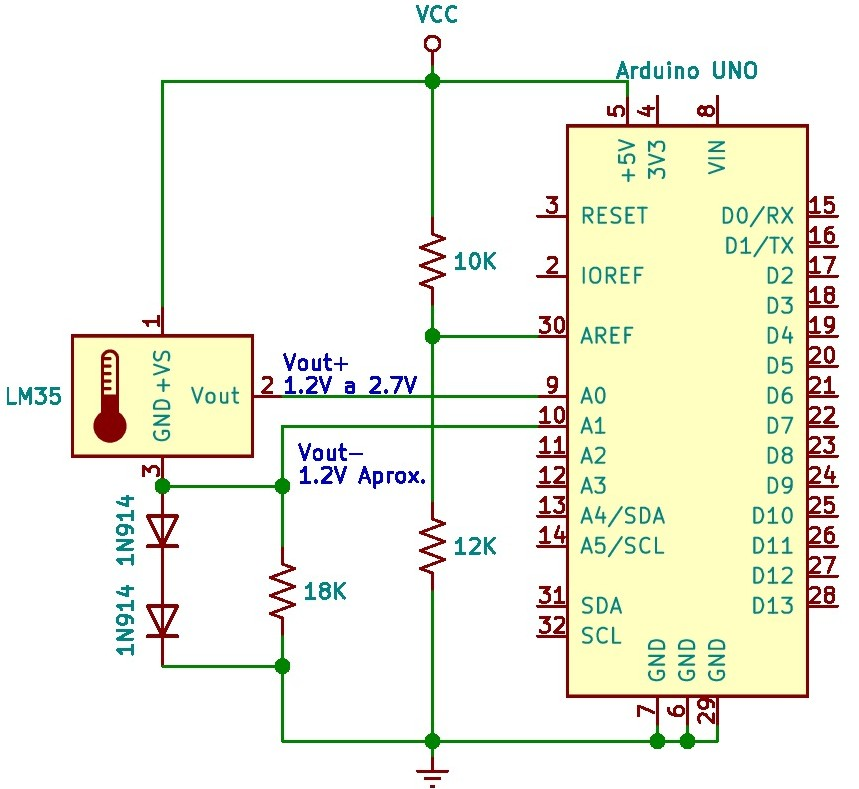
\includegraphics[width=\textwidth,height=5cm,keepaspectratio]{img/lm35-arduino.jpg}
	\caption{Circuito medidor de temperatura LM35 con Arduino}
	\label{fig:lm35-arduino} % chktex 24
\end{figure}

Con este nuevo valor de referencia se puede calcular de nueva cuenta la precisión del sensor digital una vez decodificado el valor analógico leído del LM35 dividiendo los 2.73V de referencia entre los 1024 valores posibles que entrega el ADC como sigue:

\begin{equation}
\Delta V = \frac{ 2.73V }{ 1024 } =  0.00267V
\end{equation}

Debido a que la resolución máxima del sensor LM35 determinada por su factor de incertidumbre es de \degreesC{0.5} equivalentes a 0.005V, ambas configuraciones (con y sin el divisor de voltaje) serán adecuadas para operar al sensor.